\subsubsection{Identifying input parameters}
The strength of the prediction is very much dependent on the quality of the underlying data. As described in Section~\ref{sec:dataCollection} the data must satisfy certain criteria before it can be used as input and output for the Artificial Neural Network. It must be trustworthy and contain hourly observations for our specific purposes, e.g. day-ahead wind power and electricity price prediction based on a dataset that consists of hourly observations. All calculations in the ANN are based on this data which makes it of utmost importance for the forecast. The selection of the correct input parameters for testing is equally important which is described in the analysis in Chapter~\ref{ch:theANNs}. The analysis of both electricity price and wind production together with experiment one in Sections~\ref{sec:windPowerExperimentOne} and~\ref{sec:priceExperimentOne} show how the combination of the right parameters is the core to a good prediction. It is necessary to make a comprehensive analysis of different parameters to know what to include in the experiment and how to represent them. A good example of this is the seasonal aspect for electricity prices which showed difference in result when used as month or as the specific season (summer, winter, ect.). Consequently, the pre-requisites for the wind power and electricity price experiments to perform accurately is the the quality and selection of the input data since it is the basic foundation for the Artificial Neural Network to generalize upon.

Examples of publications where the importance of analysing exactly what input parameters constitutes the electricity price, why and how they are represented is limited is in\cite{szkuta1999electricity,sansom1999neural,1} which is also discussed in Section~\ref{sec:priceExperimentThree}. A sensitivity test to identify influences have been carried out for 4 out of the 15 input in \cite{szkuta1999electricity} and there is no description of the last parameters. Article \cite{1} decided only to use only historical price data for prediction but without going into detail how it is represented. It makes it very difficult to imitate the behaviour and use or test their knowledge and experience on how to include and represent inputs in the best possible way. The seasonal aspect can as mentioned be included in different ways, matrix can be used and the combination of the inputs have very different impact. Exactly what combination of inputs and how they are represented should always be documented for others to imitate and test on own datasets so that results can be compared based on the same data. Our experiments showed that even though some inputs was closely co-related to the output it was not necessarily included in the best prediction as seen with consumption and wind power in Section~\ref{sec:windPowerExperimentOne}. The black box nature of the ANN can identify unforeseen dependencies between the various input parameters. It is not enough to simply list the characteristics of the output to predict without mentioning what came out of the input analysis, did the experiments validate it and exactly what inputs was used. The analysis is the foundation for what the experiments are suppose to validate, e.g. the various hypothesis's of experiment one are build based on the analysis. Expectations that was not met can also be explained by the analysis, for instance the substitution of consumption with air density or temperature. What influence the electricity price can differ from country to country due to different market conditions and different weather which makes it necessary to include it. In \cite{sansom1999neural} the input analysis is described with the following statement:

\begin{quotation}
\textit{The 13 inputs to the neural network were selected by data analysis and by trial and error to produce the seven-day ahead electricity price forecast. The inputs were time, demand and price data obtained from the SEM web site...}
\end{quotation}

The focus should not be on the results alone but also how the result is obtained through the dataset, especially in the case of input parameters for the neural network which have shown to be of utmost importance in our analysis. The point being that all publications use different datasets and experimental environments and in order to compare results to one another the different settings must be the same and tested on the same dataset. The lack in description of test environment and input analysis makes such comparisons difficult both due to the incomplete information but also because the format of the datasets can't be seen or downloaded to extract the information from yourself. Comparison with another publication was attempted in Section~\ref{sec:priceExperimentThree} and it showed the difficulties in comparing because we can never be certain of their experimental setup without it being properly documented --- it can be discussed if is even fair. The purpose of our thesis is amongst other things to identify the feasibility of an Artificial Neural Network used for prediction of wind power and electricity prices. The above discussion is related to this topic because the feasibility of the ANN is directly dependent on the quality and transparency of the data that it generalizes upon. The analysis that identifies the correct inputs together with the experiments to verify the best combination and network configuration is the foundation for the result and in our experience the most time-consuming, e.g. the actual analysis and how to get from there to the best possible network setting. One thing to add is how different wind power prediction is in this thesis compared to all other publications read. They take as their starting point a physical windmill or wind-farm with all information about throughput of the mill(s) whereas we try to predict the entire production for western Denmark (DK1) based on the average weather conditions, demand and historical production data. The wind power was established to be related to the market through the co-relation to demand in Section~\ref{sec:consumptionWindProduction}, but it is evident that wind power has more obvious core parameters than price. Wind will always have the most significant influence on wind power since it is what makes the blades go round whereas price will be more reliant on market forces. It does not change the need for analysing the specific conditions both because wind power is related to the market but also because the weather changes greatly from country to country, e.g. air density is much different in India~\ref{WindPowerGenerationUsingANN} and seasonality which was discarded in our experiments could play a more significant role in places with more significant changes in weather conditions than Denmark.

\subsubsection{Input combination}
As described above the different combinations of input parameters is found in experiment one for both electricity prices and wind power production. The experiments show the complexity in the black box nature of ANN since it identifies better connections of input than foreseen. In wind power production the substitution of temperature and air density with consumption showed better accuracy which was not expected, whereas wind speed showed to be much more crucial to the electricity price than foreseen. Wind power production impacts the electricity price as presented in \cite{dayAheadImpactOfWindPowerForecasts} but more than expected through the wind speed. This leads to the potential of feeding the electricity price with the prediction of wind power as input instead of wind speed to make the prediction more accurate. This connection has to be investigated in future work.

The seasonality characteristic of the wind power production and electricity price time-series is in both cases significant and for that reason expected to increase performance for both predictions. Seasonality is reflected in the month input parameter and showed different results. The month parameter obviously decreased the overall performance of the network in the case of wind power whereas it was increased in the electricity price. The first thought was the small size of the data only containing three months and therefore not reflecting the the seasons from the previous year which was the intention. When attempted on a whole years training set it showed an overall worsening in accuracy due to over-training due to the bigger training set. The electricity prices with the seasonal aspect was also tried with a training set containing a year but as opposed to wind power the accuracy of the forecasts stayed the same. What can be concluded from this is that more data is not necessarily equal to better results in both cases and 3 months of data is the most expressive to predict 24 hours ahead in our case. What was believed to be problematic was the shifting from one season to another where the new season was significantly different from the one we came from. This was proven wrong by the experiments since 3 months itself showed to contain enough information about the current season to be accurate and the the potential shortcomings from seasonal shifts were compensated by the omission of unnecessary data from the rest of the year. The high volatility results in many different cases during the year which can make it hard for the network to generalize when the data set becomes to huge.

\subsubsection{Unseen data}
\label{sec:unseenDataDiscussion}
The wind power section emphasized in connection with input parameter experiments the need for measuring accuracy of results only on the testing set (unseen data). It was seen in Table~\ref{table:predictionMAEUnseenVsTrainingSet} that the MAE could be the same across all predictions on the training set compared to a huge difference when applied on the testing set. The best MAE on unseen data showed the worst MAE on the training set. Furthermore, different seasons and consumptions during the year result in many different days where the electricity prices and wind power behaves differently. This is also discussed in the analysis in Chapter~\ref{ch:theANNs} and therefore the experiments must as a minimum be performed on an entire year of unseen data to cover all possible scenarios and thereby reflect reality. All simulations in this thesis is performed once on a year but more testing on the same year could be conducted to further validate and strengthen results. This stands opposed to the 5 weeks from different seasons used in \cite{1} which is argued to ensure fairness in results and reflect reality. A last example is in \cite{pjmForecast} where the experiments are performed on 5 different days throughout an entire year and then again on 2 weeks in February (see table results in Figure~\ref{pjmResults}). Based on these days they conclude the following:

\begin{quotation}
\textit{The test results obtained through the simulation demonstrate that the proposed algorithm is robust, efficient, and accurate, and it produces better results for any day of the week.}
\end{quotation}

Omitting 340 days and concluding that it in general obtains better results is in contrast with our analysis of the seasonal aspect because they days differ much but also the results from experiment five in Section~\ref{sec:windPowerExperimentFive} and~\ref{sec:priceExperimentFive} where various starting points during the year greatly influences the overall results. The same omitting of testing days applies for~\ref{yamin2004adaptive} where a fixed testing period of one week is used for all experiments and at the same time basis for their conclusion. According to our experiments a more comprehensive testing period must be taken into consideration due to the different days and different results when claiming the feasibility and sufficiency of the prediction. One point to bring forward from~\ref{yamin2004adaptive} is the discussion of the use of Monte Carlo to eliminate randomness by running the same experiments more than once. The ANN can give somewhat different results even though predicting the same days due to the weights being initialized randomly every time. The suggested method could be used in our experiments to strengthen the results but it could result in time becoming an issue due to the huge amount of tests already conducted. The way we try to eliminate randomness is by predicting an entire year so that all seasons are represented but at the same reducing it by predicting many similar days many times during the whole year. Running the experiments more than once could be incorporated in such a way that an amount of the best predictions in every experiment could be run several times to ensure the results, for instance top-10. 

\begin{figure}[H]
\centering
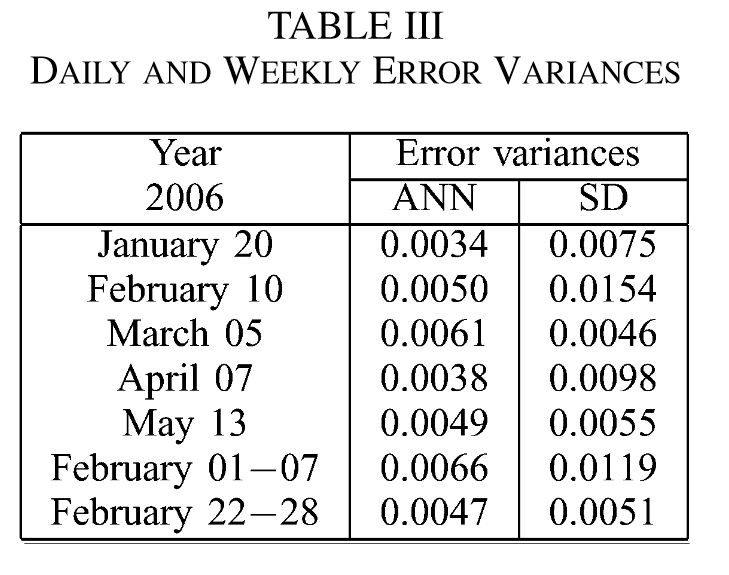
\includegraphics[width=0.99\linewidth]{billeder/pjmResults.png}
\caption{Final results from \cite{pjmForecast}}
\label{fig:pjmResults}
\end{figure}